Notes for vid10.mp4

\subsection*{Analog filters}

2 big ways to talk about analog filters: convert analog filter to
digital filter, or estimate their coefficients. 

The anlogue filter is typically easier to talk about because it lives
in the s-plane for it's transfer function:

\begin{align*}
    H(s) = \frac{B(s)}{A(s)} = 
    \frac{
        b_0 s^N + b_1 s^{N-1} \cdots + b_M
    } {
        s^N + a_1 s^{N-1} \cdots a_N s + a_N
    }
\end{align*}

\subsection*{Freq Resp}

Evaluated on the $j\omega$ axis

\begin{align*}
    H(s) \vert_s=j\omega = H(j\omega)
\end{align*}

\subsection*{Power Response}

\begin{align*}
    P(\omega) 
    &\stackrel{\Delta}{=} G^2(\omega) 
    \stackrel{\Delta}{=}
    \vert H(j \omega) \vert^2 \\
    &= H(s)H(-s)\vert_{s=j\omega} \\
    &= H(j \omega)H(-j\omega) 
    &= \overline{H(j \omega)H(-j\omega)} (real filter)
\end{align*}

For a real filter, we can fit a rational polynomial to the power response, 
and do what is called a \textit{Spectral Factorization} to find the
stable poles, and the unstable poles will be on the other side.\\

\textbf{Example LPF}\\

\paulhint{see frame 14a taken at 8:02 }\\
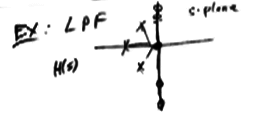
\includegraphics[scale=0.5]{frames/14a}\\
Poles will be in the left hand plane (stable). 

Zeros anywhere it wants. 
Most of the time zeros are at infinity, but more aggressive filters will have
finite zeros.

This is a lowpass filter: graphical method of the impulse response:

Start at DC, take the product of the lengths of all the zeros and take the
products of all the lengths of the poles. As you get away from the poles,
you'll be dividing by large distances to the poles.

Until you leave the "zone" of poles, it's hard to see really where the minimum 
is. 

These are the poles and zeros of $H(-s)$. 

$H(-s)$:
\paulhint{see frame 14b taken at 8:51 }\\
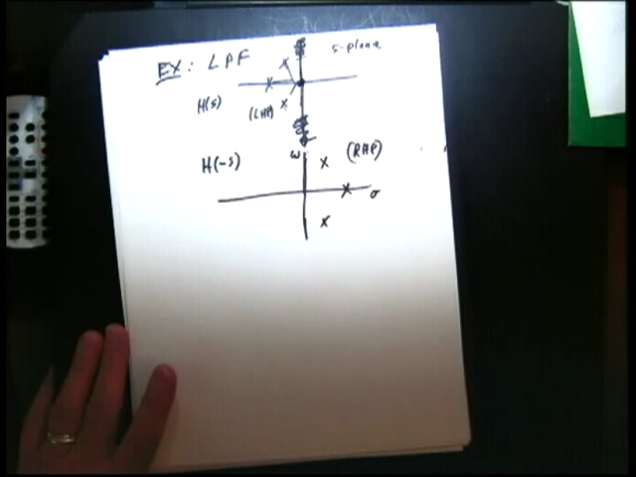
\includegraphics[scale=0.5]{frames/14b}\\

Poles exist in right half plane (RHP). Negative poles in previous graph
exist in left half plane (LHP). 

$H(-s)$: what it relfects about both sigma and the $j\omega$ axis: it's a
double flip, but there's an updown symmetry because the filter is real. Because
it's real, it has complex conjugate symmetry, so the updown flip doesn't do an thing.

\paulhint{TODO: read up on symmetry}

For real filters, you can think of them as being flipped left/right.

When you multiply, you get a symetric constellation of poles:
$H(s)H(-s)$

That is what the power response looks like for a lowpass filter. A generalized
power response. We've taken the power response and extended it to the entire 
complex plane by means of analytic continuation. 

\paulhint{See 14c at 10:22}\\
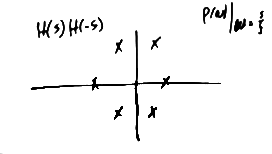
\includegraphics[scale=0.5]{frames/14c}\\

Since P is even in $\omega$, that implies that it is of the form:

\paulhint{See eqn 14d 12:03. TODO: maybe TeX this out?}\\
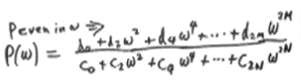
\includegraphics[scale=0.5]{frames/14d}\\

It is not going to have any odd powers of omega. 

We aren't assuming it is monic for generality. 

If there was a cubed term, there would be an asymmetry about zero on the
$j\omega$ axis, and it could not be a real filter. TO be a real filter,
it has to have a symmetric magnitiude, and you square it to get the power
response. \\

This is another example why the S-plane is easier to work in: we don't
get this on the unit circle, and we don't get this nice disapperance of
odd order terms. 

\subsection*{LPF Design}

Passband: Desired response (gain) is $P(\omega) = 1$. \\

Error: 
\begin{align*}
    E(\omega) &\stackrel{\Delta}{=} P(\omega) - 1\\
    &= \frac{D(\omega)}{C(\omega)} - 1 \\
    &= \frac{D(\omega) - C(\omega)}{C(\omega)} \\
    E(\omega)C(\omega) &= D(\omega) - C(\omega)
\end{align*}

Lets start using up degrees of freedom to get what we want. 

We can't set $E$ to zero, because there is no stop band. 

To avoid degenerecy (ie make it a lowpass) will require N > M. This means
D cannot be equal to C. \\

In audio, signals are concetrated around DC, the sampling rates are very large,
and we hear on a more or less log freq scale, and so the first octaves are
the most important. You really want to concentrate on a good filter at the low
frequencies. \\

Let $E(0) = 0 \rightarrow D(0) = C(0) \leftrightarrow d_0 = c_0$ \\

By insisting on exact unity DC gain, it's very often important that your
DC gain be exactly 1; anything greater than 1 is a growth of DC, anything less
is a loss of DC. In physical modelling, this is very important.\\

The next thing want to do is to set the slope to zero at DC: $E'(0) = 0$.

Let's differentiate it:

\paulhint{See the eqn at 14e} 
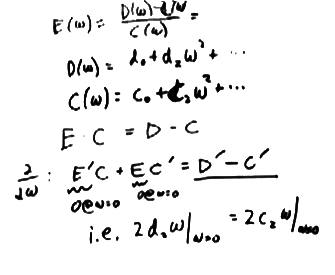
\includegraphics[scale=0.5]{frames/14e}\\

This is already true because it's even. Take the second derivitive $E''C$.

\paulhint{See the eqn at 14f 24:55} \\
\paulhint{Continuation of 14f... 14g 28:35}\\
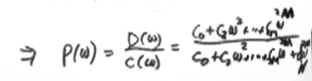
\includegraphics[scale=0.5]{frames/14f}\\

One leftover term forces it to be a lowpass. This maximizes flatness in
the pass band from DC. Flatness: how many terms in the taylor expansion you set to zero:
\begin{align*}
    0 = E(0) = E'(0) = E''(0) = \cdots 
\end{align*}

\paulhint{LOOK UP: Pade approximation}

